\section{Langkah-Langkah Percobaan}

Percobaan dilakukan dalam tiga bagian, yaitu Wireless Point-to-Point (PtP), Wireless Point-to-Multipoint (PtMP), dan Wireless Bridge, dengan menggunakan dua perangkat laptop dan dua buah router MikroTik.

\subsection{Wireless Point-to-Point (PtP)}

\begin{enumerate}
  \item Reset kedua router MikroTik.
  \item Login ke kedua router.
  \item Atur Router A sebagai \textit{Bridge} melalui menu \textit{Wireless} $\rightarrow$ \textit{WiFi interface}, dan beri nama SSID \texttt{PointToPoint\_2}.
  
\begin{figure}[H]
    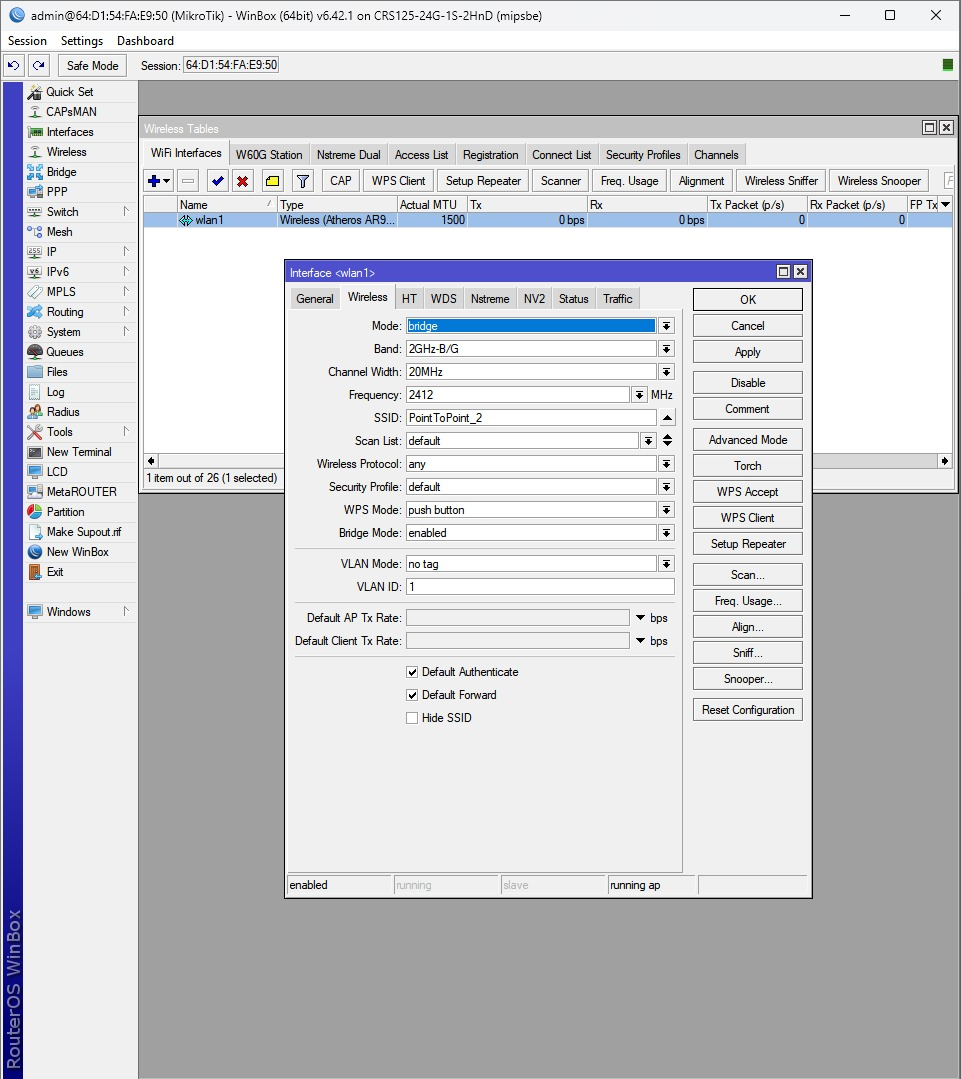
\includegraphics[width=0.48\textwidth]{P1/img/bridge.jpg}
\end{figure}

  \item Atur Router B sebagai \textit{Station}.
  \item Pada Router B, lakukan \textit{scan} untuk menemukan SSID \texttt{PointToPoint\_2}, kemudian klik \textit{connect}.
  \item Konfigurasi IP WLAN:
  \begin{itemize}
    \item Router A: \texttt{10.10.10.1/29} pada interface \texttt{wlan1}
    \item Router B: \texttt{10.10.10.2/29} pada interface \texttt{wlan1}
  \end{itemize}
  \item Konfigurasi IP LAN:
  \begin{itemize}
    \item Router A: \texttt{192.168.20.1/24} pada \texttt{ether1}
    \item Router B: \texttt{192.168.30.1/24} pada \texttt{ether1}
  \end{itemize}
  \item Konfigurasi IP laptop:
  \begin{itemize}
    \item Laptop A (Router A): \texttt{192.168.20.2/24}
    \item Laptop B (Router B): \texttt{192.168.30.2/24}
  \end{itemize}
  \item Tambahkan \textit{static routing} di kedua router melalui menu \texttt{IP → Routes}.
  
  \begin{figure}[H]
    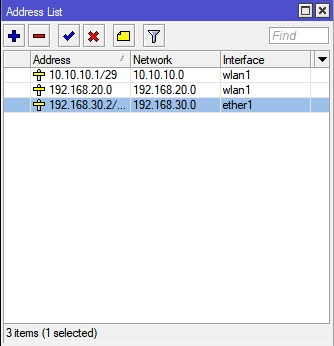
\includegraphics[width=0.48\textwidth]{P1/img/address.jpg}
\end{figure}

  \item Uji koneksi menggunakan perintah \texttt{ping} antar-router dan antar-PC.

\begin{figure}[H]
  \centering
  \begin{minipage}[t]{0.48\textwidth}
    \centering
    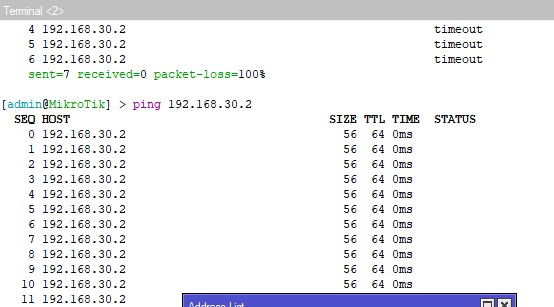
\includegraphics[width=\linewidth]{P1/img/pingrslt2.jpg}
    \caption{Ping PC to PC}
    \label{fig:production}
  \end{minipage}
  \hfill
  \begin{minipage}[t]{0.48\textwidth}
    \centering
    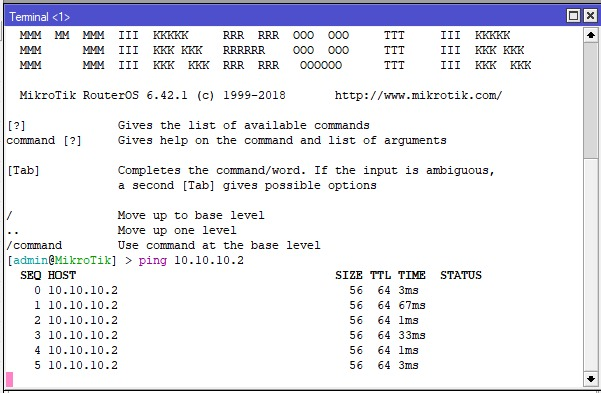
\includegraphics[width=\linewidth]{P1/img/pingrslt4.jpg}
    \caption{Ping Router to Router}
    \label{fig:admin}
  \end{minipage}
\end{figure}
  
\end{enumerate}

\subsection{Wireless Point-to-Multipoint (PtMP)}

\begin{enumerate}
  \item Reset kedua router.
  \item Login ke router.
  \item Atur Router A sebagai \textit{AP Bridge} dengan SSID \texttt{PointToPoint\_2}.
  \item Atur Router B sebagai \textit{Station}.
  \item Scan SSID \texttt{PointToPoint\_2} dari Router B, kemudian \textit{connect}.
  \item Konfigurasi IP WLAN dan LAN sama seperti PtP.
  \item Konfigurasi IP laptop sama seperti PtP.
  \item Tambahkan static route di masing-masing router.
  \item Lakukan pengujian konektivitas dengan perintah \texttt{ping}.

  \begin{figure}[H]
  \centering
  \begin{minipage}[t]{0.48\textwidth}
    \centering
    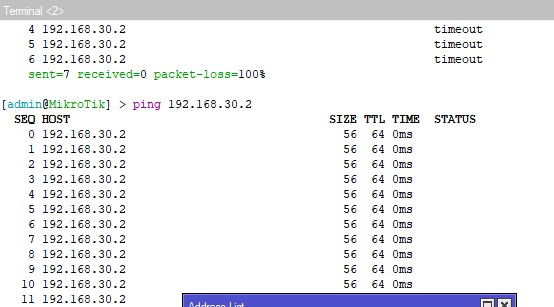
\includegraphics[width=\linewidth]{P1/img/pingrslt2.jpg}
    \caption{Ping PC to PC}
    \label{fig:production}
  \end{minipage}
  \hfill
  \begin{minipage}[t]{0.48\textwidth}
    \centering
    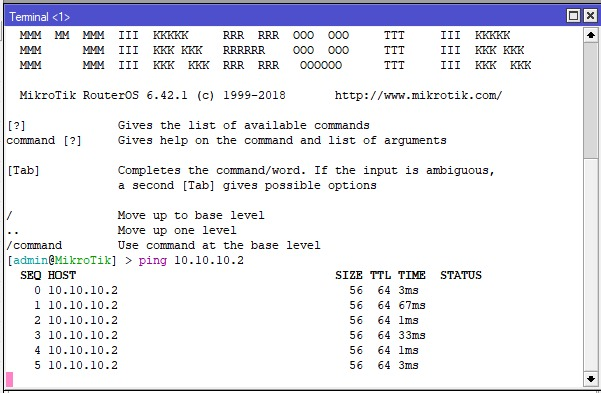
\includegraphics[width=\linewidth]{P1/img/pingrslt4.jpg}
    \caption{Ping Router to Router}
    \label{fig:admin}
  \end{minipage}
\end{figure}

\end{enumerate}

\subsection{Wireless Bridge}

\begin{enumerate}
  \item Reset router.
  \item Login ke router.
  \item Atur Router A sebagai \textit{Bridge} dengan SSID \texttt{PointToPoint\_2}.
  \item Atur Router B sebagai \textit{Station Pseudobridge}.
  \item Lakukan scan dan connect dari Router B ke Router A.
  \item Konfigurasi IP WLAN, LAN, dan laptop seperti konfigurasi sebelumnya.
  \item Tambahkan static route pada kedua router.
  \item Uji konektivitas antar-router dan antar-PC.
\end{enumerate}


\section{Analisis Hasil Percobaan}

Berdasarkan pengujian yang telah dilakukan:

\begin{itemize}
  \item Pada percobaan \textbf{Point-to-Point}, koneksi wireless berhasil menghubungkan dua router secara langsung dan stabil. PC pada masing-masing router dapat saling terhubung setelah konfigurasi routing dilakukan dengan benar.
  
  \item Pada percobaan \textbf{Point-to-Multipoint}, Router A berhasil berperan sebagai AP dan Router B sebagai station. Koneksi dapat dilakukan secara simultan dengan performa yang setara dengan konfigurasi PtP, meskipun ada sedikit delay pada saat koneksi awal.
  
  \item Pada percobaan \textbf{Wireless Bridge}, koneksi antar-router berhasil terbentuk dengan mode bridge dan station pseudobridge. Semua perangkat berada dalam satu domain broadcast, namun pengalamatan IP dan routing tetap diperlukan untuk komunikasi antar-subnet.
  
  \item Semua mode berhasil diuji melalui \texttt{ping}, baik antar-router maupun antar-PC, dengan catatan seluruh konfigurasi IP dan route telah benar. Ketika terdapat kesalahan pada pengaturan IP atau gateway, koneksi gagal dan menghasilkan \texttt{Request Timed Out}.
\end{itemize}


\section{Hasil Tugas Modul}

\subsection{Topologi Jaringan Wireless Antargedung}

Pada tugas ini telah dilakukan simulasi jaringan wireless Point-to-Multipoint (PTMP) antara tiga gedung, yaitu:

\begin{itemize}
  \item Gedung Pusat
  \item Gedung Lab
  \item Gedung Asrama (dengan dua blok: Blok A dan Blok B)
\end{itemize}

Setiap gedung diwakili oleh satu buah router \texttt{WRT300N} dan satu PC. Khusus untuk Gedung Asrama, digunakan dua buah PC mewakili Blok A dan Blok B, namun tetap menggunakan satu router untuk menjembatani koneksi keduanya secara bridge (LAN-to-LAN).'

\begin{figure}[H]
  \centering
  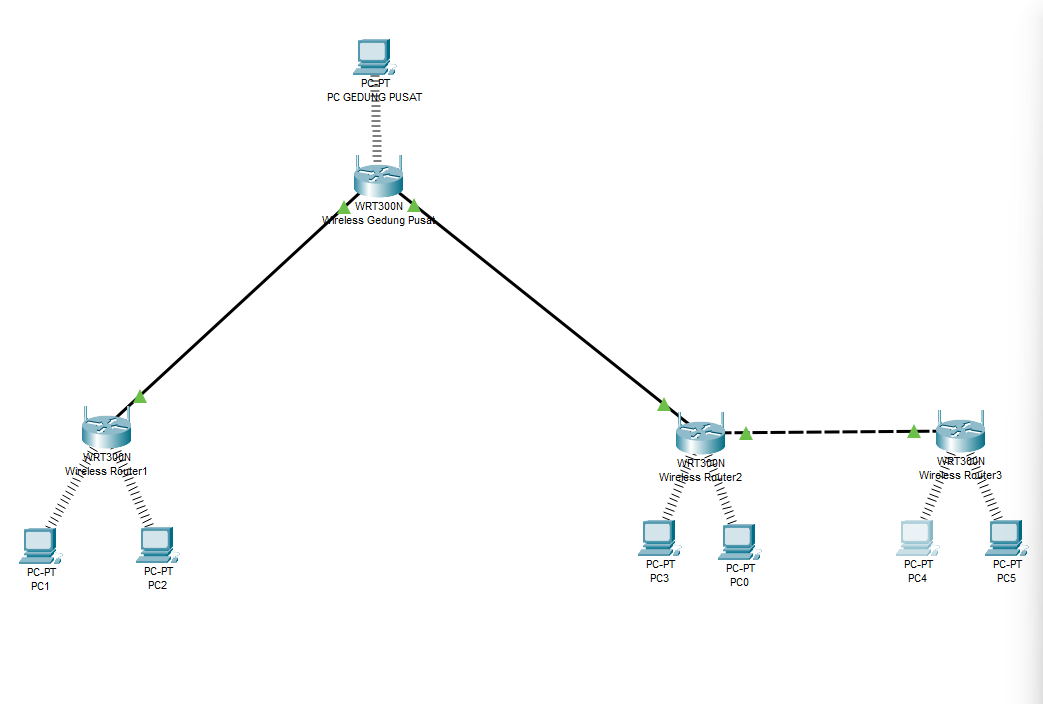
\includegraphics[width=0.48\textwidth]{P1/img/Topologi.png}
  \caption{Seluruh Jaringan terkoneksi}
  \label{fig:connected}
\end{figure}

\subsection{Konfigurasi Router Pusat}

\begin{itemize}
  \item \textbf{Internet Setup}
  \begin{itemize}
    \item Connection Type: Static IP
    \item IP Address: 10.0.0.1
    \item Subnet Mask: 255.255.255.0
    \item Default Gateway: (kosong atau dummy jika tidak koneksi luar)
  \end{itemize}
  
  \item \textbf{Network Setup}
  \begin{itemize}
    \item IP Address: 192.168.1.1
    \item Subnet Mask: 255.255.255.0
    \item DHCP Server: Enabled
    \item Start IP Address: 192.168.1.10
    \item Maximum Users: 50
  \end{itemize}
  
  \item \textbf{Wireless Setup}
  \begin{itemize}
    \item SSID: JaringanPusat
    \item Wireless Mode: Mixed
    \item SSID Broadcast: Enabled
  \end{itemize}
  
  \item \textbf{Wireless Security}
  \begin{itemize}
    \item Mode: WPA2 Personal
    \item Password: admin123
  \end{itemize}
\end{itemize}

\subsection{Konfigurasi Router Gedung Lain (Lab dan Asrama)}

Setiap router selain pusat (Lab, Asrama) dikonfigurasi sebagai access point (bridge) dengan pengaturan:

\begin{itemize}
  \item \textbf{Internet Setup}
    \begin{itemize}
      \item IP Address: 10.0.0.2 (Lab), 10.0.0.3 (Asrama A), 10.0.0.4 (Asrama B)
      \item Subnet Mask: 255.255.255.0
      \item Default Gateway: 10.0.0.1 (Router Pusat)
    \end{itemize}
  
  \item \textbf{Network Setup (LAN)}
    \begin{itemize}
      \item IP Address: 192.168.1.2 (Lab), 192.168.1.3 (Asrama A), 192.168.1.4 (Asrama B)
      \item DHCP Server: Disabled
    \end{itemize}
    
  \item \textbf{Wireless Setup}
    \begin{itemize}
      \item SSID: Sama dengan Router Pusat untuk roaming (JaringanPusat)
      \item Wireless Security: Sama (WPA2 Personal, admin123)
    \end{itemize}
    
  \item \textbf{Koneksi antar Router}
    \begin{itemize}
      \item Router Pusat terhubung ke semua router gedung via kabel (LAN ke LAN atau LAN ke Internet port tergantung mode)
      \item Blok A dan B Asrama dihubungkan LAN-to-LAN
    \end{itemize}
\end{itemize}

\subsection{Pengujian Jaringan}

Pengujian dilakukan dengan perintah \texttt{ping} dari masing-masing PC:

\begin{itemize}
  \item Ping antar PC dalam satu gedung berhasil
  \item Setelah konfigurasi bridge dan IP diperbaiki, ping antar gedung juga berhasil
  \item DHCP hanya aktif di Router Pusat dan berhasil mendistribusikan IP ke semua PC
\end{itemize}

\begin{figure}[H]
  \centering
  \begin{minipage}[t]{0.48\textwidth}
    \centering
    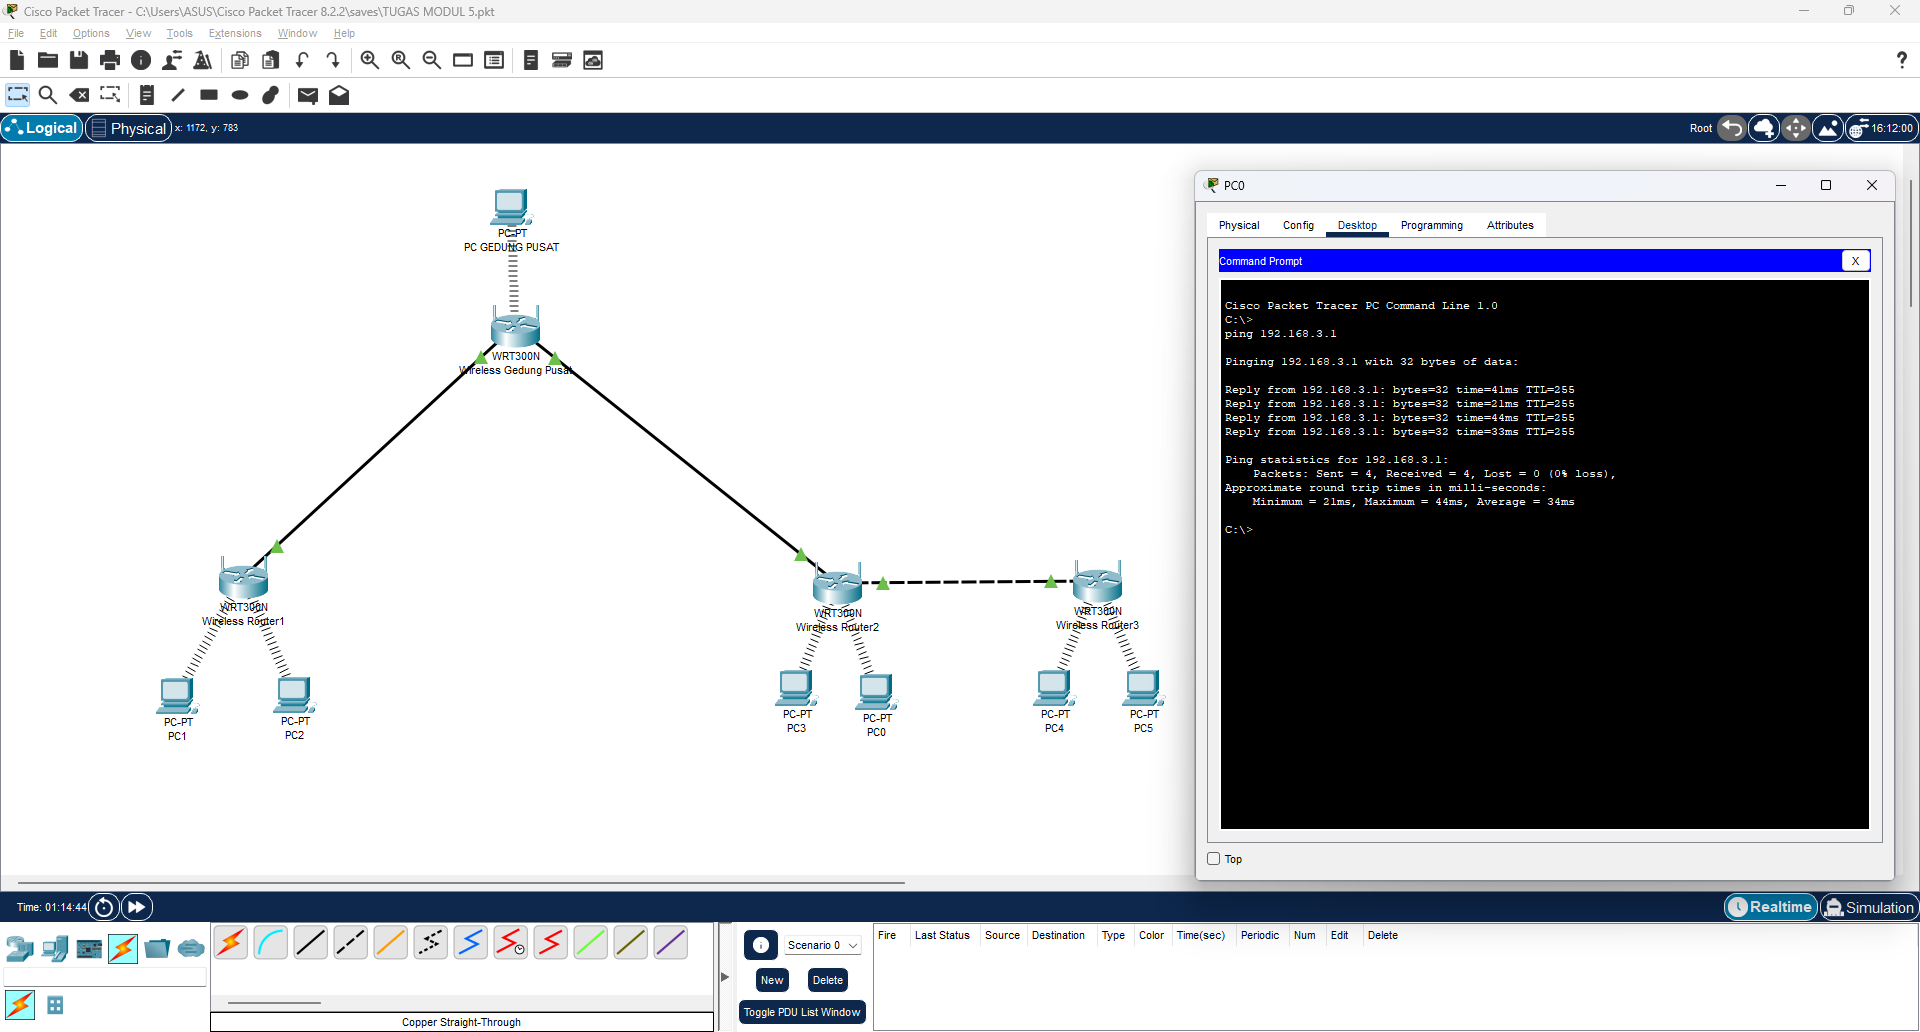
\includegraphics[width=\linewidth]{P1/img/Test Ping PC ke Router.png}
    \caption{Ping PC to Router}
    \label{fig:production}
  \end{minipage}
  \hfill
  \begin{minipage}[t]{0.48\textwidth}
    \centering
    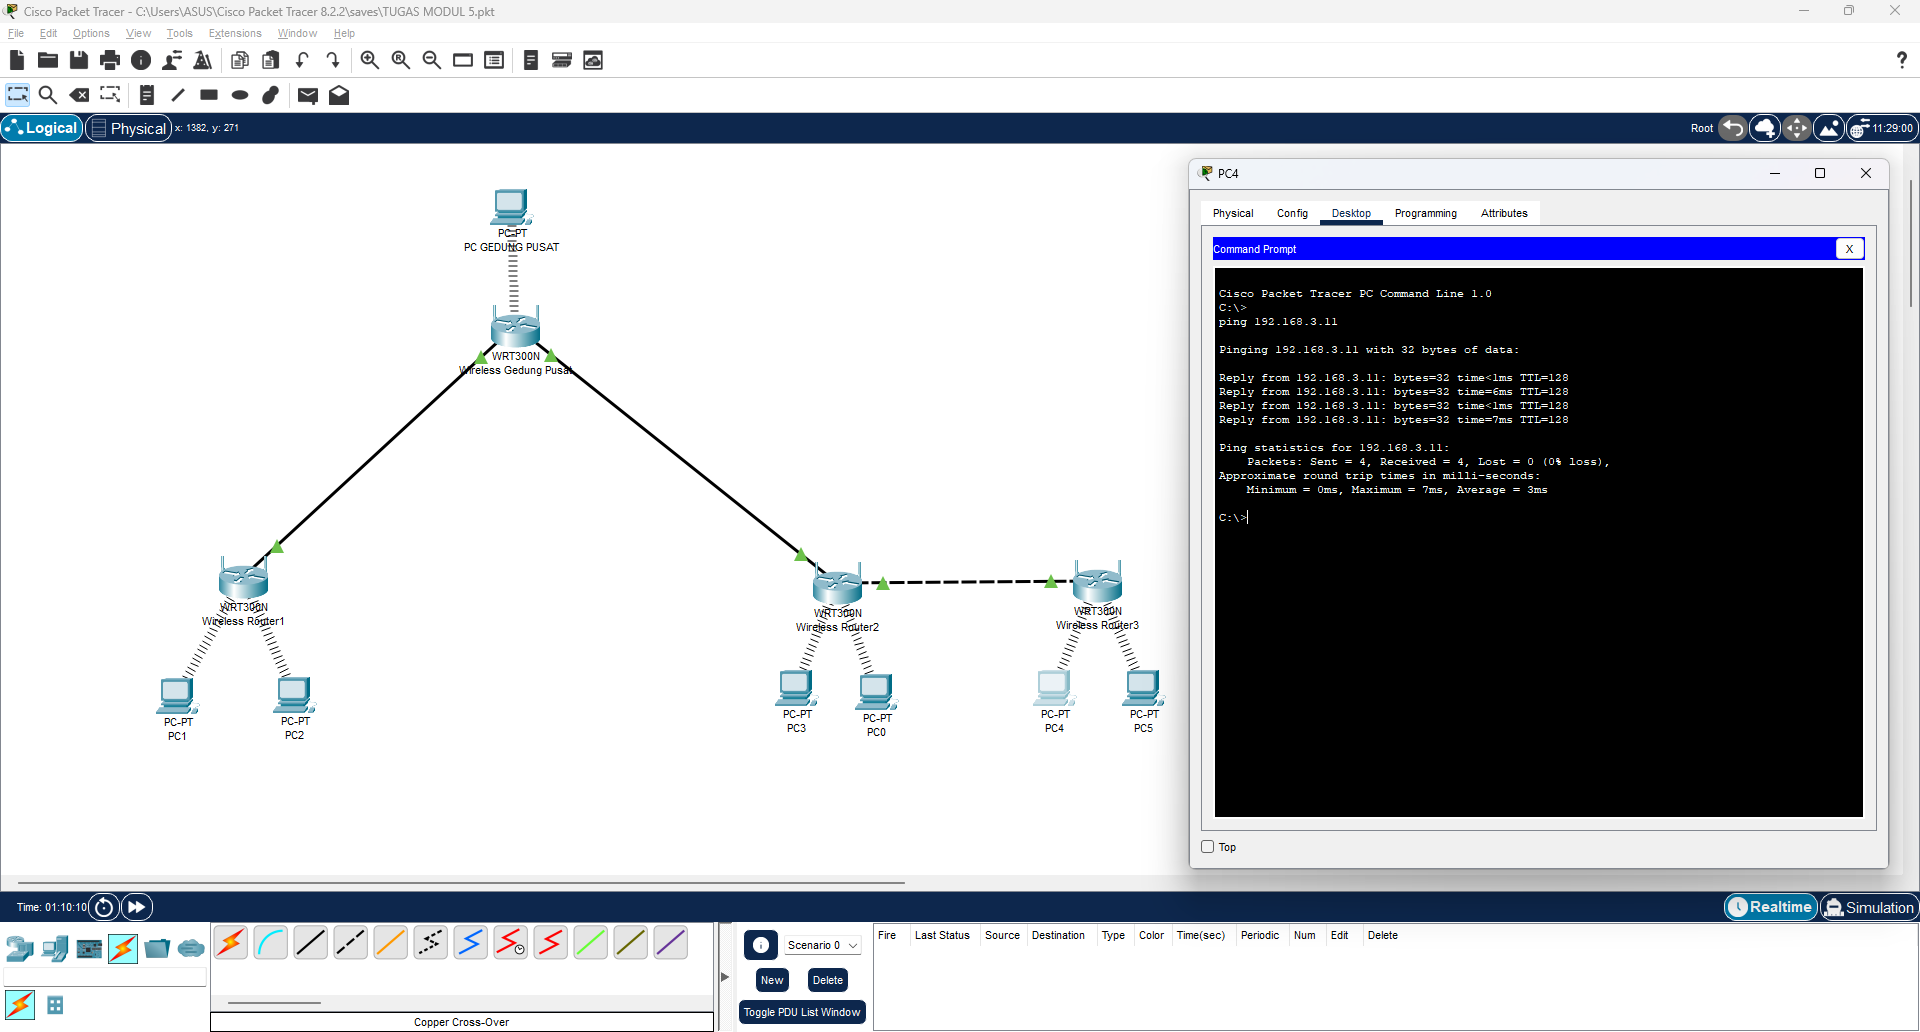
\includegraphics[width=\linewidth]{P1/img/Test Ping Antar PC.png}
    \caption{Ping PC to PC}
    \label{fig:admin}
  \end{minipage}
\end{figure}


\section{Kesimpulan}

Dari percobaan yang telah dilakukan, dapat disimpulkan bahwa:

\begin{itemize}
  \item Wireless LAN dapat dibangun dengan berbagai metode seperti Point-to-Point, Point-to-Multipoint, dan Wireless Bridge, sesuai dengan kebutuhan topologi jaringan.
  
  \item Penggunaan mode \textit{bridge} atau \textit{station pseudobridge} memungkinkan integrasi jaringan layer 2, sementara mode routing tetap membutuhkan konfigurasi IP dan static routing.
  
  \item Keberhasilan komunikasi antar perangkat sangat bergantung pada ketepatan konfigurasi IP, gateway, dan routing.
  
  \item MikroTik RouterOS memberikan fleksibilitas tinggi dalam membangun topologi wireless, termasuk dalam pengaturan interface, wireless mode, hingga manajemen IP dan routing.
\end{itemize}
